\documentclass[journal,12pt,onecolumn]{IEEEtran}
\usepackage{cite}
 \usepackage{caption}
\usepackage{graphicx}
\usepackage{amsmath,amssymb,amsfonts,amsthm}
\usepackage{algorithmic}
\usepackage{graphicx}
\usepackage{textcomp}
\usepackage{xcolor}
\usepackage{txfonts}
\usepackage{listings}
\usepackage{enumitem}
\usepackage{mathtools}
\usepackage{gensymb}
\usepackage{comment}
\usepackage[breaklinks=true]{hyperref}
\usepackage{tkz-euclide} 
\usepackage{listings}
\usepackage{gvv}
%\def\inputGnumericTable{}                                 
\usepackage[latin1]{inputenc} 
\usetikzlibrary{arrows.meta, positioning}
\usepackage{xparse}
\usepackage{color}                                            
\usepackage{array}                                            
\usepackage{longtable}                                       
\usepackage{calc}                                             
\usepackage{multirow}
\usepackage{multicol}
\usepackage{hhline}                                           
\usepackage{ifthen}                                           
\usepackage{lscape}
\usepackage{tabularx}
\usepackage{array}
\usepackage{float}

\usepackage{float}
%\newcommand{\define}{\stackrel{\triangle}{=}}
\theoremstyle{remark}
\usepackage{circuitikz}
\captionsetup{justification=centering}
\usepackage{tikz}

\title{Matrices in Geometry 4.13.40}
\author{EE25BTECH11035 - Kushal B N}
\begin{document}
\vspace{3cm}
\maketitle
{\let\newpage\relax\maketitle}
\textbf{Question: }\\
The number of integer values of $m$ for which the x-coordinate of the point of intersection of the lines $3x + 4y = 9$ and $y = mx + 1$ is also an integer, is
\begin{multicols}{4}
\begin{enumerate}
    \item 2
    \item 0
    \item 4
    \item 1
\end{enumerate}
\end{multicols}

\textbf{Given: } \\
The two lines\\
$\myvec{3&4}\myvec{x\\y}=9$ and $\myvec{m&-1}\myvec{x\\y}=-1$

\textbf{Solution: }\\
The given set of equations can be written as,
\begin{equation}
    \myvec{3&4\\m&-1}\myvec{x\\y} = \myvec{9\\-1}
\end{equation}

Augmented Matrix:
\begin{equation}
    \myvec{3&4&|&9\\m&-1&|&-1}
\end{equation}

\begin{equation}
    \myvec{3&4&|&9\\m&-1&|&-1} \overset{R_2 \rightarrow R_2 - \frac{m}{3}R_1}{\longrightarrow} \myvec{3&4&|&9\\0&-1-\frac{4m}{3}&|&-1-3m}
\end{equation}

\begin{equation}
    \implies y = 3\brak{\frac{3m+1}{4m+3}}
\end{equation}

\begin{equation}
    \implies x = \frac{5}{4m+3}
\end{equation}
Thus, for $x$ to be an integer, while keeping the denominator also an integer,\\
\begin{equation}
\brak{4m+3} \in \cbrak{1,5,-1,-5}
\end{equation}

\begin{equation}
    \implies m \in \cbrak{\frac{-1}{2},\frac{1}{2},-1,-2}
\end{equation}

Hence, for m to be an integer value $m = -1$ or $m = -2$.

\textbf{Conclusion: }\\
$\therefore$ There are 2 integer values of $m$ for which the x-coordinate of the point of intersection of the given lines is also an integer.\\
Hence, the correct answer is option (1).

\begin{figure}[H]
    \centering
    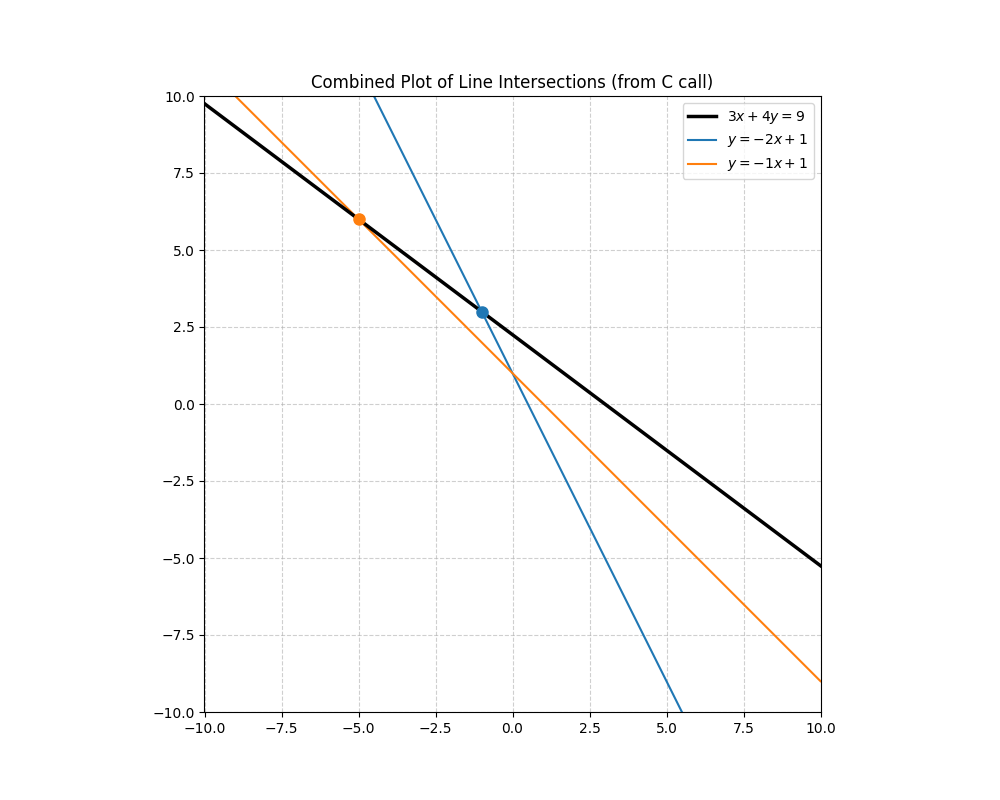
\includegraphics[width=0.75\columnwidth]{figs/1.png}
    \caption{}
\end{figure}

\end{document}

